\mfpicnumber{1}

\opengraphsfile{LogEquations}

\setcounter{footnote}{0}

\label{LogEquations}

In Section \ref{ExpEquations} we solved equations and inequalities involving exponential functions using one of two basic strategies.  We now turn our attention to equations and inequalities involving logarithmic functions, and not surprisingly, there are two basic strategies to choose from.  For example, suppose we wish  to solve $\log_{2}(x) = \log_{2}(5)$.  Theorem \ref{explogsonetoone} tells us that the \textit{only} solution to this equation is $x=5$.  Now suppose we wish to solve $\log_{2}(x) = 3$.  If we want to use Theorem \ref{explogsonetoone}, we need to rewrite $3$ as a logarithm base $2$.   We can use Theorem \ref{invpropslogs} to do just that: $3 = \log_{2}\left(2^{3}\right) = \log_{2}(8)$.  Our equation then becomes  $\log_{2}(x) =  \log_{2}(8)$ so that $x = 8$.  However, we could have arrived at the same answer,  in fewer steps, by using Theorem \ref{invpropslogs} to rewrite the equation $\log_{2}(x) = 3$ as $2^{3} = x$, or $x=8$.  We summarize the two common ways to solve log equations below.

\smallskip

\colorbox{ResultColor}{\bbm

\centerline{\textbf{Steps for Solving an Equation involving Logarithmic Functions}} \index{logarithm ! solving equations with} 

\begin{enumerate}

\item  Isolate the logarithmic function.

\item  \begin{enumerate}

\item  If convenient, express both sides as logs with the same base and equate the arguments of the log functions.

\item  Otherwise, rewrite the log equation as an exponential equation.


\end{enumerate}

\end{enumerate}

\ebm}

\smallskip

\begin{ex}  \label{LogEqnsEx1} Solve the following equations.  Check your solutions graphically using a calculator.

\begin{multicols}{2}
\begin{enumerate}

\item  $\log_{117}(1-3x) = \log_{117}\left(x^2-3\right)$

\item  $2 - \ln(x-3) = 1$

\setcounter{HW}{\value{enumi}}
\end{enumerate}
\end{multicols}

\begin{multicols}{2}
\begin{enumerate}
\setcounter{enumi}{\value{HW}}

\item  $\log_{6}(x+4) + \log_{6}(3-x) = 1$

\item  $\log_{7}(1-2x) = 1 - \log_{7}(3-x)$
\setcounter{HW}{\value{enumi}}
\end{enumerate}
\end{multicols}

\begin{multicols}{2}
\begin{enumerate}
\setcounter{enumi}{\value{HW}}

\item  $\log_{2}(x+3) = \log_{2}(6-x)+3$

\item  $1 + 2 \log_{4}(x+1) = 2 \log_{2}(x)$

\end{enumerate}
\end{multicols}

{\bf Solution.}

\begin{enumerate}

\item  Since we have the same base on both sides of the equation $\log_{117}(1-3x) = \log_{117}\left(x^2-3\right)$, we equate what's inside the logs to get $1-3x = x^2-3$.  Solving $x^2+3x-4 = 0$ gives $x=-4$ and $x=1$. To check these answers using the calculator, we make use of the change of base formula and graph $f(x) = \frac{\ln(1-3x)}{\ln(117)}$ and $g(x) = \frac{\ln\left(x^2-3\right)}{\ln(117)}$ and we see they intersect only at $x=-4$.  To see what happened to the solution $x=1$, we substitute it into our original equation to obtain  $\log_{117}(-2) =  \log_{117}(-2)$.  While these expressions look identical, neither is a real number,\footnote{They do, however, represent the same \textbf{family} of complex numbers.  We stop ourselves at this point and refer the reader to a good course in Complex Variables.} which means $x=1$ is not in the domain of the original equation, and is not a solution.    

\item  Our first objective in solving $2 - \ln(x-3) = 1$ is to isolate the logarithm.  We get $\ln(x-3)=1$, which, as an exponential equation, is $e^{1} = x-3$.  We get our solution $x=e+3$. On the calculator, we see the graph of $f(x) = 2 - \ln(x-3)$ intersects  the graph of $g(x) = 1$ at $x = e+3 \approx 5.718$.

\begin{center}

\begin{tabular}{cc}

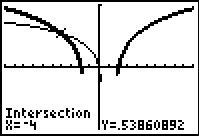
\includegraphics[width=2in]{./ExpLogsGraphics/LogEqns01.jpg} &

\hspace{0.75in} 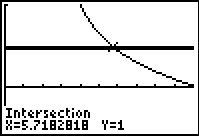
\includegraphics[width=2in]{./ExpLogsGraphics/LogEqns02.jpg} \\

$y = f(x) =\log_{117}(1-3x)$ and   & 

 \hspace{0.75in}  $y = f(x) =  2 - \ln(x-3)$ and \\
 
 \boldmath $y=g(x) =\log_{117}\left(x^2-3\right)$ & 
 \hspace{0.75in} \boldmath $y=g(x) = 1$  \\

\end{tabular}

\end{center}

\item We can start solving $\log_{6}(x+4) + \log_{6}(3-x) = 1$ by using the Product Rule for logarithms to rewrite the equation as  $\log_{6}\left[(x+4)(3-x)\right] = 1$.  Rewriting this as an exponential equation, we get $6^{1} = (x+4)(3-x)$.  This reduces to $x^2+x-6 = 0$, which gives $x=-3$ and $x=2$.   Graphing $y=f(x) =  \frac{\ln(x+4)}{\ln(6)} + \frac{\ln(3-x)}{\ln(6)}$ and $y=g(x) = 1$, we see they intersect twice, at $x=-3$ and $x=2$.

\begin{center}

\begin{tabular}{cc}

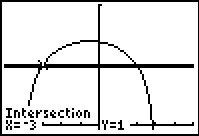
\includegraphics[width=2in]{./ExpLogsGraphics/LogEqns03.jpg} &

\hspace{0.75in} 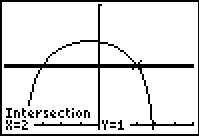
\includegraphics[width=2in]{./ExpLogsGraphics/LogEqns04.jpg} \\

\end{tabular}

$y = f(x) =\log_{6}(x+4) + \log_{6}(3-x)$ and  \boldmath  $y=g(x) = 1$

\end{center}

\item  Taking a cue from the previous problem, we begin solving $\log_{7}(1-2x) = 1 - \log_{7}(3-x)$ by first collecting the logarithms on the same side, $\log_{7}(1-2x) +  \log_{7}(3-x) = 1$, and then using the Product Rule to get $\log_{7}[(1-2x)(3-x)] = 1$.  Rewriting this as an exponential equation gives $7^{1} = (1-2x)(3-x)$ which gives the quadratic equation $2x^2-7x-4=0$.  Solving, we find  $x = -\frac{1}{2}$ and $x=4$.  Graphing, we find $y = f(x) = \frac{\ln(1-2x)}{\ln(7)}$ and $y=g(x) = 1 - \frac{\ln(3-x)}{\ln(7)}$ intersect only at $x=-\frac{1}{2}$.  Checking $x=4$ in the original equation produces $\log_{7}(-7) = 1 - \log_{7}(-1)$, which is a clear domain violation.

\item Starting with  $\log_{2}(x+3) = \log_{2}(6-x)+3$, we gather the logarithms to one side and get $\log_{2}(x+3) - \log_{2}(6-x) = 3$.  We then use the Quotient Rule and convert to an exponential equation \[\log_{2}\left(\frac{x+3}{6-x}\right) = 3 \iff 2^{3} = \frac{x+3}{6-x} \] This reduces to the linear equation $8(6-x) = x+3$, which gives us $x = 5$.  When we graph $f(x) = \frac{\ln(x+3)}{\ln(2)}$ and $g(x) =  \frac{\ln(6-x)}{\ln(2)} + 3$, we find they intersect at $x=5$.

\begin{center}

\begin{tabular}{cc}

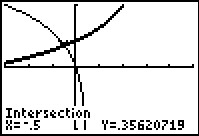
\includegraphics[width=2in]{./ExpLogsGraphics/LogEqns05.jpg} &

\hspace{0.75in} 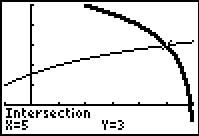
\includegraphics[width=2in]{./ExpLogsGraphics/LogEqns06.jpg} \\

$y = f(x) =\log_{7}(1-2x)$ and   & 

 \hspace{0.75in}  $y = f(x) =  \log_{2}(x+3)$ and \\
 
 \boldmath $y=g(x)=1 - \log_{7}(3-x)$ & 
 \hspace{0.75in} \boldmath $y=g(x) = \log_{2}(6-x)+3$  \\

\end{tabular}

\end{center}

\item Starting with $1 + 2 \log_{4}(x+1) = 2 \log_{2}(x)$, we gather the logs to one side to get the equation $1 = 2 \log_{2}(x) - 2 \log_{4}(x+1)$.  Before we can combine the logarithms, however, we need a common base.  Since $4$ is a power of $2$, we use change of base to convert  \[\log_{4}(x+1) = \frac{\log_{2}(x+1)}{\log_{2}(4)} = \frac{1}{2} \log_{2}(x+1)\] Hence, our original equation becomes  

\[ \begin{array}{rclr}

1 & = & 2 \log_{2}(x) - 2 \left(\frac{1}{2} \log_{2}(x+1)\right) & \\ [2pt]
1 &= & 2\log_{2}(x) - \log_{2}(x+1) & \\ [2pt]
1 & = & \log_{2}\left(x^2\right) - \log_{2}(x+1) & \text{Power Rule} \\ [6pt]
1 & = & \log_{2}\left( \dfrac{x^{2}}{x+1}\right) & \text{Quotient Rule} \\ \end{array}\]

Rewriting this in exponential form, we get $ \frac{x^{2}}{x+1} = 2$ or $x^2 -2x-2 = 0$.  Using the quadratic formula, we get $x = 1 \pm \sqrt{3}$.  Graphing $f(x) = 1 + \frac{2\ln(x+1)}{\ln(4)}$ and $g(x) = \frac{2 \ln(x)}{\ln(2)}$, we see the graphs intersect only at $x = 1 + \sqrt{3} \approx 2.732$.  The solution $x = 1 - \sqrt{3} < 0$, which means if substituted into the original equation, the term $2 \log_{2}\left(1 - \sqrt{3}\right)$ is undefined.

\begin{center}
\begin{tabular}{c}

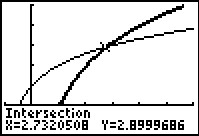
\includegraphics[width=2in]{./ExpLogsGraphics/LogEqns07.jpg} \\

$y = f(x) = 1 + 2 \log_{4}(x+1)$ and \boldmath $y = g(x) = 2 \log_{2}(x)$ \\

\end{tabular}
\end{center}
\end{enumerate}

\qed
\end{ex}

If nothing else,  Example \ref{LogEqnsEx1} demonstrates the importance of checking for extraneous solutions\footnote{Recall that an extraneous solution is an answer obtained analytically which does not satisfy the original equation.} when solving equations involving logarithms.  Even though we checked our answers graphically, extraneous solutions are easy to spot - any supposed solution which causes a negative number inside a logarithm needs to be discarded.  As with the equations in Example \ref{expeqnsex1}, much can be learned from checking all of the answers in Example \ref{LogEqnsEx1} analytically.  We leave this to the reader and turn our attention to inequalities involving logarithmic functions.  Since logarithmic functions are continuous on their domains, we can use sign diagrams.  

\begin{ex}  Solve the following inequalities.  Check your answer graphically using a calculator.
\label{logineq}

\begin{multicols}{3}

\begin{enumerate}

\item  $\dfrac{1}{\ln(x)+1} \leq 1$

\item  $\left(\log_{2}(x)\right)^2 < 2 \log_{2}(x) + 3$

\item  $x \log(x+1) \geq x$


\end{enumerate}

\end{multicols}


{\bf Solution.}  

\begin{enumerate}

\item  We start solving $\frac{1}{\ln(x)+1} \leq 1$ by getting $0$ on one side of the inequality: $\frac{1}{\ln(x)+1}  - 1 \leq 0$.  Getting a common denominator yields $\frac{1}{\ln(x)+1}  - \frac{\ln(x)+1}{\ln(x)+1} \leq 0$ which reduces to $\frac{-\ln(x)}{\ln(x)+1} \leq 0$, or $ \frac{\ln(x)}{\ln(x)+1} \geq 0$.  We define $r(x) = \frac{\ln(x)}{\ln(x)+1}$ and set about finding the domain and the zeros of $r$.  Due to the appearance of the term $\ln(x)$, we require  $x > 0$.  In order to keep the denominator away from zero, we solve $\ln(x)+1 = 0$ so $\ln(x) = -1$, so $x = e^{-1} = \frac{1}{e}$.  Hence, the domain of $r$ is $\left(0, \frac{1}{e}\right) \cup \left(\frac{1}{e}, \infty\right)$.  To find the zeros of $r$, we set $r(x) = \frac{\ln(x)}{\ln(x)+1} = 0$ so that $\ln(x) = 0$, and we find $x = e^{0} = 1$.  In order to determine test values for $r$ without resorting to the calculator, we need to find numbers between $0$, $\frac{1}{e}$, and $1$ which have a base of $e$.  Since $e \approx 2.718 > 1$, $0 < \frac{1}{e^2} < \frac{1}{e} < \frac{1}{\sqrt{e}} < 1 < e$.  To determine the sign of $r\left( \frac{1}{e^2} \right)$, we use the fact that $\ln\left(\frac{1}{e^2}\right) = \ln\left(e^{-2}\right) = -2$, and find $r\left( \frac{1}{e^2} \right) = \frac{-2}{-2+1} = 2$, which is $(+)$.  The rest of the test values are determined similarly.   From our sign diagram, we find the solution to be $\left(0, \frac{1}{e}\right) \cup [1, \infty)$. Graphing $f(x) =  \frac{1}{\ln(x)+1}$ and $g(x) = 1$, we see the graph of $f$ is below the graph of $g$ on the solution intervals, and that the graphs intersect at $x=1$.

\begin{center}

\begin{tabular}{m{2in}c}

\begin{mfpic}[10]{-6}{6}{-2}{2}
\arrow \polyline{(-6,0),(6,0)}
\xmarks{-6,-2,2}
\tiny
\tlpointsep{6pt}
\normalsize
\tlabel[cc](-6,-1){$0$}
\tlabel[cc](-4,1){$(+)$}
\tlabel[cc](-2,-1){$\frac{1}{e}$}
\tlabel[cc](-2,1){\textinterrobang}
\tlabel[cc](0,1){$(-)$}
\tlabel[cc](2,-1){$1$}
\tlabel[cc](2,1){$0$}
\tlabel[cc](4,1){$(+)$}
\end{mfpic} 

& 

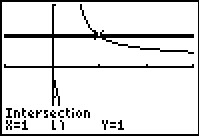
\includegraphics[width=2in]{./ExpLogsGraphics/LogEqns08.jpg} \\

& $y=f(x) = \frac{1}{\ln(x)+1}$ and \boldmath $y = g(x) = 1$ \\

\end{tabular}

\end{center}

\item  Moving all of the nonzero terms of  $\left(\log_{2}(x)\right)^2 < 2 \log_{2}(x) + 3$ to one side of the inequality, we have $\left(\log_{2}(x)\right)^2 - 2 \log_{2}(x) - 3 < 0$. Defining $r(x) = \left(\log_{2}(x)\right)^2 - 2 \log_{2}(x) - 3$, we get the domain of $r$ is $(0, \infty)$, due to the presence of the logarithm.  To find the zeros of $r$, we set $r(x) =\left(\log_{2}(x)\right)^2 - 2 \log_{2}(x) - 3= 0$ which results in a `quadratic in disguise.'  We set $u = \log_{2}(x)$ so our equation becomes $u^2-2u-3 = 0$ which gives us $u=-1$ and $u=3$.  Since $u = \log_{2}(x)$, we get $\log_{2}(x) = -1$, which gives us $x = 2^{-1} = \frac{1}{2}$, and $\log_{2}(x) = 3$, which yields $x = 2^{3} = 8$.  We use test values which are powers of $2$: $0 < \frac{1}{4} < \frac{1}{2} < 1 < 8 < 16$, and from our sign diagram, we see $r(x)< 0$ on $\left(\frac{1}{2}, 8 \right)$. Geometrically, we see the graph of $f(x)= \left(\frac{\ln(x)}{\ln(2)}\right)^2$ is below  the graph of $y = g(x) = \frac{2 \ln(x)}{\ln(2)} + 3$ on the solution interval.

\begin{center}

\begin{tabular}{m{2in}c}

\begin{mfpic}[10]{-6}{6}{-2}{2}
\arrow \polyline{(-6,0),(6,0)}
\xmarks{-6,-2,2}
\tiny
\tlpointsep{6pt}
\normalsize
\tlabel[cc](-6,-1){$0$}
\tlabel[cc](-4,1){$(+)$}
\tlabel[cc](-2,-1){$\frac{1}{2}$}
\tlabel[cc](-2,1){$0$}
\tlabel[cc](0,1){$(-)$}
\tlabel[cc](2,-1){$8$}
\tlabel[cc](2,1){$0$}
\tlabel[cc](4,1){$(+)$}
\end{mfpic} 

& 

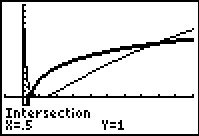
\includegraphics[width=2in]{./ExpLogsGraphics/LogEqns09.jpg} \\

& $y=f(x) = \left(\log_{2}(x)\right)^2$ and \boldmath $y = g(x) = 2 \log_{2}(x) + 3$ \\

\end{tabular}

\end{center}

\item  We begin to solve $x \log(x+1) \geq x$ by subtracting $x$ from both sides to get $x \log(x+1)  - x \geq 0$.  We define $r(x) = x \log(x+1)  - x $ and due to the presence of the logarithm, we require $x+1 > 0$, or $x > -1$.  To find the zeros of $r$, we set $r(x) = x \log(x+1)  - x = 0$.  Factoring, we get $x \left(\log(x+1) - 1\right) = 0$, which gives $x=0$ or $\log(x+1) - 1=0$.  The latter gives $\log(x+1) = 1$, or $x+1 = 10^{1}$, which admits $x = 9$.  We select test values $x$ so that $x+1$ is a power of $10$, and we obtain $-1 < -0.9 < 0 < \sqrt{10} -1 < 9 < 99$.  Our sign diagram gives the solution to be $(-1,0] \cup [9, \infty)$. The calculator indicates the graph of $y= f(x) = x \log(x+1)$ is above $y=g(x) = x$ on the solution intervals, and the graphs intersect at $x=0$ and $x=9$.


\begin{center}

\begin{tabular}{m{2in}c}

\begin{mfpic}[10]{-6}{6}{-2}{2}
\arrow \polyline{(-6,0),(6,0)}
\xmarks{-6,-2,2}
\tiny
\tlpointsep{4pt}
\normalsize
\tlabel[cc](-6,-1){$-1$}
\tlabel[cc](-4,1){$(+)$}
\tlabel[cc](-2,-1){$0$}
\tlabel[cc](-2,1){$0$}
\tlabel[cc](0,1){$(-)$}
\tlabel[cc](2,-1){$9$}
\tlabel[cc](2,1){$0$}
\tlabel[cc](4,1){$(+)$}
\end{mfpic} 

& 

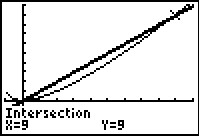
\includegraphics[width=2in]{./ExpLogsGraphics/LogEqns10.jpg} \\

& $y=f(x) = x \log(x+1)$ and \boldmath $y = g(x) = x$ \\

\end{tabular}

\end{center} 

\end{enumerate}

\qed

\end{ex}

\smallskip

Our next example revisits the concept of pH first seen in Exercise \ref{pHexercise} in Section \ref{IntroExpLogs}.  


\begin{ex}

In order to successfully breed Ippizuti fish the pH of a freshwater tank must be at least 7.8 but can be no more than 8.5.  Determine the corresponding range of hydrogen ion concentration, and check your answer using a calculator.

\smallskip

{\bf Solution.}  Recall from Exercise \ref{pHexercise} in Section \ref{IntroExpLogs} that $\mbox{pH} = -\log[\mbox{H}^{+}]$ where $[\mbox{H}^{+}]$ is the hydrogen ion concentration in moles per liter.  We require $7.8 \leq -\log[\mbox{H}^{+}] \leq 8.5$ or $-7.8 \geq \log[\mbox{H}^{+}] \geq -8.5$.  To solve this compound inequality we solve $-7.8 \geq \log[\mbox{H}^{+}]$ and $ \log[\mbox{H}^{+}] \geq -8.5$ and take the intersection of the solution sets.\footnote{Refer to page \pageref{intersectionunion} for a discussion of what this means.}  The former inequality yields $0 < [\mbox{H}^{+}] \leq 10^{-7.8}$ and the latter yields $[\mbox{H}^{+}] \geq 10^{-8.5}$.  Taking the intersection gives us our final answer $10^{-8.5} \leq [\mbox{H}^{+}] \leq 10^{-7.8}$.  (Your Chemistry professor may want the answer written as $3.16 \times 10^{-9} \leq [\mbox{H}^{+}] \leq 1.58 \times 10^{-8}$.)  After carefully adjusting the viewing window on the graphing calculator we see that the graph of $f(x) = -\log(x)$ lies between the lines $y = 7.8$ and $y = 8.5$ on the interval $[3.16 \times 10^{-9}, 1.58 \times 10^{-8}]$.

\smallskip

\begin{center}

\begin{tabular}{cc}

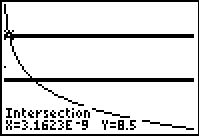
\includegraphics[width=2in]{./ExpLogsGraphics/LogEqns13.jpg}  \hspace{0.75in} & 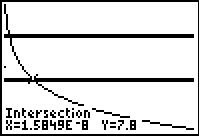
\includegraphics[width=2in]{./ExpLogsGraphics/LogEqns14.jpg}  \\

\end{tabular}

\end{center}

\centerline{The graphs of $y = f(x) = -\log(x)$, \boldmath $y = 7.8$ and \boldmath $y = 8.5$}

\qed

\end{ex}

\smallskip

We close this section by finding an inverse of a one-to-one function which involves logarithms.

\begin{ex}  \label{logfracinverse} The function $f(x) = \dfrac{\log(x)}{1-\log(x)}$ is one-to-one.  Find a formula for $f^{-1}(x)$ and check your answer graphically using your calculator.

{\bf Solution.}  We first write $y=f(x)$ then interchange the $x$ and $y$ and solve for $y$.

\[ \begin{array}{rclr}
y & = & f(x) & \\ 
y  & = & \dfrac{\log(x)}{1-\log(x)} & \\[8pt]
x  & = & \dfrac{\log(y)}{1-\log(y)} & \mbox{Interchange $x$ and $y$.}\\[8pt]
x\left(1-\log(y)\right) & = & \log(y) & \\ 
x - x\log(y)  & = & \log(y) & \\ 
x & = & x \log(y) + \log(y) & \\ 
x & = & (x+1) \log(y) & \\ 
\dfrac{x}{x+1}  & = & \log(y) & \\ 
y & = & 10^{\frac{x}{x+1}} & \mbox{Rewrite as an exponential equation.}\\

\end{array}\]

\pagebreak

We have $f^{-1}(x) = 10^{\frac{x}{x+1}}$.  Graphing $f$ and $f^{-1}$ on the same viewing window yields

\begin{center}
\begin{tabular}{c}

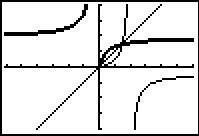
\includegraphics[width=2in]{./ExpLogsGraphics/LogEqns15.jpg} \\

$y = f(x) = \dfrac{\log(x)}{1-\log(x)}$ and \boldmath $y = g(x) = 10^{\frac{x}{x+1}}$ \\

\end{tabular}
\end{center}

\qed

\end{ex}

\newpage
\subsection{Exercises}

In Exercises \ref{solvelogeqexfirst} - \ref{solvelogeqexlast}, solve the equation analytically.

\begin{multicols}{2}
\begin{enumerate}

\item $\log(3x-1) = \log(4-x)$  \label{solvelogeqexfirst}

\item $\log_{2}\left(x^{3}\right) = \log_{2}(x)$

\setcounter{HW}{\value{enumi}}
\end{enumerate}
\end{multicols}

\begin{multicols}{2}
\begin{enumerate}
\setcounter{enumi}{\value{HW}}

\item $\ln\left(8-x^2\right)=\ln(2-x)$

\item $\log_{5}\left(18-x^2\right) = \log_{5}(6-x)$

\setcounter{HW}{\value{enumi}}
\end{enumerate}
\end{multicols}

\begin{multicols}{2}
\begin{enumerate}
\setcounter{enumi}{\value{HW}}

\item $\log_{3}(7-2x) = 2$
\item $\log_{\frac{1}{2}} (2x-1) = -3$

\setcounter{HW}{\value{enumi}}
\end{enumerate}
\end{multicols}

\begin{multicols}{2}
\begin{enumerate}
\setcounter{enumi}{\value{HW}}

\item $\ln\left(x^2-99\right) = 0$
\item $\log(x^2-3x) = 1$

\setcounter{HW}{\value{enumi}}
\end{enumerate}
\end{multicols}

\begin{multicols}{2}
\begin{enumerate}
\setcounter{enumi}{\value{HW}}

\item $\log_{125} \left(\dfrac{3x-2}{2x+3}\right)=\dfrac{1}{3}$

\item $\log\left(\dfrac{x}{10^{-3}}\right) = 4.7$ \vphantom{$\log_{125} \left(\dfrac{3x-2}{2x+3}\right)$} \label{sixfourRichterequ}


\setcounter{HW}{\value{enumi}}
\end{enumerate}
\end{multicols}


\begin{multicols}{2}
\begin{enumerate}
\setcounter{enumi}{\value{HW}}

\item $-\log(x) = 5.4$ \vphantom{$10\log\left(\dfrac{x}{10^{-12}}\right)$} \label{sixfourpHequ}
\item $10\log\left(\dfrac{x}{10^{-12}}\right) = 150$ \label{sixfourdecibelequ}

\setcounter{HW}{\value{enumi}}
\end{enumerate}
\end{multicols}

\begin{multicols}{2}
\begin{enumerate}
\setcounter{enumi}{\value{HW}}

\item $6-3\log_{5}(2x)=0$
\item $3\ln(x)-2=1-\ln(x)$

\setcounter{HW}{\value{enumi}}
\end{enumerate}
\end{multicols}

\begin{multicols}{2}
\begin{enumerate}
\setcounter{enumi}{\value{HW}}

\item $\log_{3}(x - 4) + \log_{3}(x + 4) = 2$

\item $\log_{5}(2x + 1) + \log_{5}(x + 2) = 1$

\setcounter{HW}{\value{enumi}}
\end{enumerate}
\end{multicols}

\begin{multicols}{2}
\begin{enumerate}
\setcounter{enumi}{\value{HW}}

\item $\log_{169}(3x + 7) - \log_{169}(5x - 9) = \dfrac{1}{2}$

\item $\ln(x+1) - \ln(x) = 3$ \vphantom{$\log_{169}(3x + 7)$}

\setcounter{HW}{\value{enumi}}
\end{enumerate}
\end{multicols}

\begin{multicols}{2}
\begin{enumerate}
\setcounter{enumi}{\value{HW}}

\item $2\log_{7}(x) = \log_{7}(2) + \log_{7}(x+12)$

\item $\log(x) - \log(2) = \log(x+8)  - \log(x+2)$

\setcounter{HW}{\value{enumi}}
\end{enumerate}
\end{multicols}

\begin{multicols}{2}
\begin{enumerate}
\setcounter{enumi}{\value{HW}}

\item $\log_{3}(x) = \log_{\frac{1}{3}}(x) + 8$

\item $\ln(\ln(x)) = 3$

\setcounter{HW}{\value{enumi}}
\end{enumerate}
\end{multicols}

\begin{multicols}{2}
\begin{enumerate}
\setcounter{enumi}{\value{HW}}

\item $\left(\log(x)\right)^2=2\log(x)+15$

\item $\ln(x^{2}) = (\ln(x))^{2}$ \label{solvelogeqexlast}

\setcounter{HW}{\value{enumi}}
\end{enumerate}
\end{multicols}


In Exercises \ref{solvelogineqexfirst} - \ref{solvelogineqexlast}, solve the inequality analytically.

\begin{multicols}{2}
\begin{enumerate}
\setcounter{enumi}{\value{HW}}

\item $\dfrac{1 - \ln(x)}{x^{2}} < 0$ \label{solvelogineqexfirst}
\item $x\ln(x) - x > 0$ \phantom{$\dfrac{1 - \ln(x)}{x^{2}} < 0$}


\setcounter{HW}{\value{enumi}}
\end{enumerate}
\end{multicols}

\begin{multicols}{2}
\begin{enumerate}
\setcounter{enumi}{\value{HW}}

\item $10\log\left(\dfrac{x}{10^{-12}}\right) \geq 90$ \label{sixfourdecibelineq} 
\item $5.6 \leq \log\left(\dfrac{x}{10^{-3}}\right) \leq 7.1$ \label{sixfourRichterineq}


\setcounter{HW}{\value{enumi}}
\end{enumerate}
\end{multicols}

\begin{multicols}{2}
\begin{enumerate}
\setcounter{enumi}{\value{HW}}


\item $2.3 < -\log(x) < 5.4$ \label{sixfourpHineq} 

\item $\ln(x^{2}) \leq (\ln(x))^{2}$ \label{solvelogineqexlast} 

\setcounter{HW}{\value{enumi}}
\end{enumerate}
\end{multicols}

In Exercises \ref{logeqcalcexfirst} - \ref{logeqcalcexlast}, use your calculator to help you solve the equation or  inequality.

\begin{multicols}{2}
\begin{enumerate}
\setcounter{enumi}{\value{HW}}

\item $\ln(x) = e^{-x}$ \label{logeqcalcexfirst} 
\item $\ln(x) = \sqrt[4]{x}$ 

\setcounter{HW}{\value{enumi}}
\end{enumerate}
\end{multicols}

\begin{multicols}{2}
\begin{enumerate}
\setcounter{enumi}{\value{HW}}

\item $\ln(x^{2} + 1) \geq 5$
\item $\ln(-2x^{3} - x^{2} + 13x - 6) < 0$ \label{logeqcalcexlast} 

\setcounter{HW}{\value{enumi}}
\end{enumerate}
\end{multicols}

\begin{enumerate}
\setcounter{enumi}{\value{HW}}

\item \label{onetooneexpexercise} Since $f(x) = e^{x}$ is a strictly increasing function, if $a < b$ then $e^{a} < e^{b}$.  Use this fact to solve the inequality $\ln(2x + 1) < 3$ without a sign diagram. Use this technique to solve the inequalities in Exercises \ref{sixfourdecibelineq} - \ref{sixfourpHineq}. (Compare this to Exercise  \ref{onetoonelogexercise} in Section \ref{ExpEquations}.)

\item Solve $\ln(3 - y) - \ln(y) = 2x + \ln(5)$ for $y$.

\item In Example \ref{logfracinverse} we found the inverse of $f(x) = \dfrac{\log(x)}{1-\log(x)}$ to be $f^{-1}(x) = 10^{\frac{x}{x+1}}$.

\begin{enumerate}

\item Show that $\left(f^{-1} \circ f\right)(x) = x$ for all $x$ in the domain of $f$ and that $\left(f \circ f^{-1}\right)(x) = x$ for all $x$ in the domain of $f^{-1}$.

\item Find the range of $f$ by finding the domain of $f^{-1}$.

\item Let $g(x) = \dfrac{x}{1 - x}$ and $h(x) = \log(x)$.  Show that $f = g \circ h$ and $(g \circ h)^{-1} = h^{-1} \circ g^{-1}$.\\
(We know this is true in general by Exercise \ref{fcircginverse} in Section \ref{InverseFunctions}, but it's nice to see a specific example of the property.)

\end{enumerate}

\item \label{inversehyptangent} Let $f(x) = \dfrac{1}{2}\ln\left(\dfrac{1 + x}{1 - x}\right)$.  Compute $f^{-1}(x)$ and find its domain and range.

\item Explain the equation in Exercise \ref{sixfourRichterequ} and the inequality in Exercise \ref{sixfourRichterineq} above in terms of the Richter scale for earthquake magnitude.  (See Exercise \ref{Richterexercise} in Section \ref{IntroExpLogs}.)

\item Explain the equation in Exercise \ref{sixfourdecibelequ} and the inequality in Exercise \ref{sixfourdecibelineq} above in terms of sound intensity level as measured in decibels.  (See Exercise \ref{decibelexercise} in Section \ref{IntroExpLogs}.)

\item Explain the equation in Exercise \ref{sixfourpHequ} and the inequality in Exercise \ref{sixfourpHineq} above in terms of the pH of a solution.  (See Exercise \ref{pHexercise} in Section \ref{IntroExpLogs}.)

\item With the help of your classmates, solve the inequality $\sqrt[n]{x} > \ln(x)$ for a variety of natural numbers $n$.  What might you conjecture about the ``speed'' at which $f(x) = \ln(x)$ grows versus any principal $n^{\textrm{th}}$ root function?

\end{enumerate}

\newpage

\subsection{Answers}
\begin{multicols}{3}
\begin{enumerate}

\item $x = \frac{5}{4}$
\item $x = 1$
\item $x=-2$

\setcounter{HW}{\value{enumi}}
\end{enumerate}
\end{multicols}

\begin{multicols}{3}
\begin{enumerate}
\setcounter{enumi}{\value{HW}}

\item $x=-3,\, 4$
\item $x=-1$
\item $x=\frac{9}{2}$

\setcounter{HW}{\value{enumi}}
\end{enumerate}
\end{multicols}

\begin{multicols}{3}
\begin{enumerate}
\setcounter{enumi}{\value{HW}}

\item $x=\pm 10$
\item $x=-2,\, 5$
\item $x = -\frac{17}{7}$

\setcounter{HW}{\value{enumi}}
\end{enumerate}
\end{multicols}

\begin{multicols}{3}
\begin{enumerate}
\setcounter{enumi}{\value{HW}}

\item $x = 10^{1.7}$
\item $x = 10^{-5.4}$
\item $x = 10^{3}$

\setcounter{HW}{\value{enumi}}
\end{enumerate}
\end{multicols}

\begin{multicols}{3}
\begin{enumerate}
\setcounter{enumi}{\value{HW}}

\item $x=\frac{25}{2}$
\item $x=e^{3/4}$
\item $x = 5$

\setcounter{HW}{\value{enumi}}
\end{enumerate}
\end{multicols}

\begin{multicols}{3}
\begin{enumerate}
\setcounter{enumi}{\value{HW}}

\item $x = \frac{1}{2}$
\item $x = 2$
\item $x = \frac{1}{e^3-1}$

\setcounter{HW}{\value{enumi}}
\end{enumerate}
\end{multicols}

\begin{multicols}{3}
\begin{enumerate}
\setcounter{enumi}{\value{HW}}

\item $x=6$
\item $x=4$
\item $x = 81$

\setcounter{HW}{\value{enumi}}
\end{enumerate}
\end{multicols}

\begin{multicols}{3}
\begin{enumerate}
\setcounter{enumi}{\value{HW}}

\item $x = e^{e^3}$
\item $x=10^{-3}, \, 10^{5}$
\item $x = 1, \, x = e^{2}$

\setcounter{HW}{\value{enumi}}
\end{enumerate}
\end{multicols}

\begin{multicols}{3}
\begin{enumerate}
\setcounter{enumi}{\value{HW}}

\item $(e, \infty)$
\item $(e, \infty)$
\item $\left[10^{-3}, \infty \right)$

\setcounter{HW}{\value{enumi}}
\end{enumerate}
\end{multicols}

\begin{multicols}{3}
\begin{enumerate}
\setcounter{enumi}{\value{HW}}

\item $\left[10^{2.6}, 10^{4.1}\right]$

\item $\left(10^{-5.4}, 10^{-2.3}\right)$
\item $(0, 1] \cup [e^{2}, \infty)$

\setcounter{HW}{\value{enumi}}
\end{enumerate}
\end{multicols}

\begin{multicols}{2}
\begin{enumerate}
\setcounter{enumi}{\value{HW}}

\item $x \approx 1.3098$
\item $x \approx 4.177, \, x \approx 5503.665$

\setcounter{HW}{\value{enumi}}
\end{enumerate}
\end{multicols}

\begin{multicols}{2}
\begin{enumerate}
\setcounter{enumi}{\value{HW}}

\item $\approx (-\infty, -12.1414) \cup (12.1414, \infty)$
\item $\approx (-3.0281, -3) \cup (0.5, 0.5991) \cup (1.9299, 2)$

\setcounter{HW}{\value{enumi}}
\end{enumerate}
\end{multicols}

\begin{multicols}{2}
\begin{enumerate}
\setcounter{enumi}{\value{HW}}

\item $-\dfrac{1}{2} < x < \dfrac{e^{3} - 1}{2}$

\item $y = \dfrac{3}{5e^{2x} + 1}$ \vphantom{$\dfrac{e^{3} - 1}{2}$}

\setcounter{HW}{\value{enumi}}
\end{enumerate}
\end{multicols}

\begin{enumerate}
\setcounter{enumi}{\value{HW}}
\addtocounter{enumi}{1}

\item $f^{-1}(x) = \dfrac{e^{2x} - 1}{e^{2x} + 1} = \dfrac{e^{x} - e^{-x}}{e^{x} + e^{-x}}$. (To see why we rewrite this in this form, see  Exercise \ref{andtheresthyperbolic} in Section \ref{Parametric}.)  The domain of $f^{-1}$ is $(-\infty, \infty)$ and its range is the same as the domain of $f$, namely $(-1, 1)$.

\end{enumerate}

\closegraphsfile